\documentclass[conference]{IEEEtran}

\IEEEoverridecommandlockouts %To add sponsors and index terms

\usepackage{cite}

\ifCLASSINFOpdf
   \usepackage[pdftex]{graphicx}
  % declare the path(s) where your graphic files are
%   \graphicspath{{../images/}}
  % and their extensions so you won't have to specify these with
  % every instance of \includegraphics
   \DeclareGraphicsExtensions{.pdf,.jpeg,.png}
\else
\fi

\usepackage[cmex10]{amsmath}
%\usepackage[hidelinks]{hyperref}
\usepackage{nohyperref}
\usepackage{url}
%for columns spanning multiple rows in tables
\usepackage{multirow}
%use the booktabs package to get (much!) better vertical spacing above and below "rules" (horizontal lines), resulting in a much more professional look of your tables.
%use the colortbl package to add color to tables.
\usepackage{booktabs,colortbl}

\usepackage{amsfonts}

% correct bad hyphenation here
\hyphenation{op-tical net-works semi-conduc-tor}

  \renewcommand\footnoterule{\vspace*{-3pt}%
     \hrule width 2in height 0.4pt
     \vspace*{2.6pt}}

\begin{document}
%
% paper title
% can use linebreaks \\ within to get better formatting as desired
\title{Temporal Instanton Analysis:\\
Development and Implementation}


% author names and affiliations
% use a multiple column layout for up to two different
% affiliations
\author{%

\IEEEauthorblockN{Jonas Kersulis,\\ Ian Hiskens}
%\IEEEauthorblockA{Electrical Engineering and Computer Science\\
\IEEEauthorblockA{Elec. Eng. and Computer Science \\
University of Michigan\\
Ann Arbor, MI, United States\\}
\and
\IEEEauthorblockN{Michael Chertkov,\\Scott Backhaus}
%\IEEEauthorblockA{Center for Nonlinear Studies\\
\IEEEauthorblockA{Center for Nonlinear Studies\\
Los Alamos National Laboratory\\
Los Alamos, NM, United States\\
}
\and
\IEEEauthorblockN{Daniel Bienstock\\ \hspace{1pt} }
%\IEEEauthorblockA{Industrial Engineering and Operations Research\\
\IEEEauthorblockA{Ind. Eng. and Operations Research\\
Columbia University\\
New York, NY, United States\\
}

% use \thanks{} to gain access to the first footnote area
% a separate \thanks must be used for each paragraph as LaTeX2e's \thanks
% was not built to handle multiple paragraphs

% Who are our sponsors?
%\thanks{Identify applicable sponsor/s here. \emph{(sponsors)}}%
\thanks{The authors acknowledge the support of the Los Alamos National Laboratory Grid Science Program, subcontract 270958.}%
}

% make the title area
\maketitle

%ABSTRACT
\begin{abstract}
%A time-coupled instanton method for characterizing transmission network vulnerability to wind generation fluctuation is presented. To extend prior instanton work to multiple-time-step analysis, line constraints are specified in terms of temperature rather than current. An optimization formulation is developed to express the minimum wind forecast deviation such that at least one line is driven to its thermal limit. Results are shown for an IEEE RTS-96 system with several wind-farms.
A previously-developed method for studying a transmission network's vulnerability to wind forecast inaccuracy is expanded. This method uses optimization to find a wind generation pattern close to the forecast that violates a specified line. Repeating the optimization for all lines in the network yields a set of generation patterns which may be sorted by likelihood. Instanton analysis thus yields insight into the potential effects of wind forecast inaccuracy at the system level.
% To demonstrate the practicability of this method, we present results for the RTS-96 and show how the method scales to larger networks.
\end{abstract}

%INDEX TERMS
% The author shall provide up to 4 keywords (in alphabetical order) to help identify the major topics of the paper. The thesaurus of IEEE indexing keywords is posted at http://www.ieee.org/organizations/pubs/ani_prod/keywrd98.txt
\begin{IEEEkeywords}
Forecast uncertainty, Optimization, Transmission operations, Wind energy
\end{IEEEkeywords}


\section{Introduction and review}\label{sec:intro}

The impact of wind forecast inaccuracy is greater than ever in grids around the world. As reliance on wind generation increases, changes in weather can induce network congestion. In certain cases this congestion may even cause a transmission line to overheat and sag. System operators use wind forecast data to steer the network away from these scenarios, but wind forecasts are significantly less accurate than generation and demand predictions. How might forecast inaccuracies compound across the network to overheat transmission lines? How likely is this to occur? Temporal instanton analysis helps answer these questions by identifying troublesome wind patterns and ranking them according to likelihood. With this information, system operators and planners may better prepare for renewable generation uncertainty.

The instanton problem was initially considered in \cite{chertkov2011}
and \cite{chertkov2011a} where a DC power flow approximation was used
to turn instanton analysis into a convex problem with an analytic
solution. The physically accurate AC power flow formulation was used
in \cite{baghsorkhi2012}, with an iterative scheme required for
finding instanton candidates. Current instanton research is exploring
the trade-off between problem complexity and solution accuracy, with
the goal of developing the most accurate model that remains convex
(and therefore guarantees a solution).  Instanton work to date has
focused on instantaneous vulnerability by seeking to find the smallest
wind generation change that drives a line to its power or current
limit. Thus, the troublesome wind patterns uncovered by such instanton
analysis may be fleeting.

It is safe to temporarily operate a line above its current
limit. Transmission system operators know this and periodically allow
lines to operate above their limits to promote smooth operation under
heavy, though temporary, flow patterns (see the introduction of
\cite{banakar2005} for a history of dynamic line rating starting in
the 1970s). It takes time for line conductors to heat sufficiently
that they sag to an unacceptable level (as defined by statute and
nearby tree limbs). As long as the line is allowed to cool before
reaching this point, no harm will be done. If an operator is
comfortable with temporarily overloaded lines, information from
existing instanton analysis may be too conservative to aid decision
making.

In this paper we expound on temporal instanton analysis. The line temperature model we use is derived from \cite{ieee2013}. Ohmic loss heating is related to power flow angle differences according to a relationship from \cite{almassalkhi2014}. By modeling line temperature over an appropriate time horizon, the proposed method discovers multiple-time-step wind patterns that are both likely to occur and sure to induce excessive sag for at least one line in the network.

The remainder of this paper is organized as follows. Section \ref{sec:models} describes the models at the core of temporal instanton analysis. Section \ref{sec:qcqp} combines these models into a quadratically-constrained quadratic program (QCQP). The solution of this QCQP is described in Section \ref{sec:solution}. Section \ref{sec:implementation}  contains results for two networks: a modified version of the RTS-96 and the larger WECC network. The former network has been used in previous instanton analysis studies, while the latter serves to demonstrate scalability of temporal instanton analysis. Finally, an appendix contains a detailed description of the thermal model used to calculate line temperature.

We expand on prior work by providing a more detailed treatment of the objective function, discussing implementation details including computational complexity and sparsity, and proposing a particular algorithm for solving the secular equation.

%The prevalence of renewables in modern transmission networks has
%researchers and system operators asking: What happens when the wind
%changes, and could fluctuations harm the grid? The instanton problem
%provides an answer, and this paper extends instanton analysis to the
%temporal setting. Though small deviations from wind forecasts are
%typically harmless, it is possible for certain wind generation
%patterns to drive the system to an insecure operating point. Out of
%all troublesome wind generation patterns, the one that deviates least
%from the forecast is called the instanton. Instanton analysis uses
%optimization to find the set of troublesome wind patterns, each of
%which causes a particular line to encounter its flow limit. By
%ranking these wind patterns according to distance from forecast, we
%can characterize the system's vulnerability to forecast inaccuracy and
%enhance system operator awareness.
%

%The remainder of the paper describes the temporal instanton problem (Section \ref{sec:problem}), translates it into an optimization problem (Section \ref{sec:optimization}), presents a solution method (Section \ref{sec:solution}), and illustrates temporal instanton analysis using a modified RTS-96 network (Section \ref{sec:results}).
%Instanton analysis may also be viewed as an optimal control problem. The goal is to drive the system to the edge of its feasible operating region while minimizing the ``effort'' of wind variation. We want to find the smallest deviation from a wind forecast that will drive enough current through at least one line to send it to its thermal limit. It is easy to check whether a particular wind forecast will lead to a line exceeding its thermal threshold; instanton analysis provides us with the sensitivity of line overloads to changes in the given forecast.
%If the relationship between generation and heat input was linear, we would have a linear optimal control problem.


%% Wind forecast overview & justification of covariance matrix
%Wind forecasting is a complicated business. Consider first a single wind farm whose output is forecast for some future time. Let the forecast performance be represented by a random variable. Using historical data from ERCOT in Texas, \cite{hodge2011} determined appropriate density functions for this variable based on the forecast horizon. For predictions a few minutes or hours away, forecast performance is approximately Cauchy, with deviations concentrated heavily around the forecast value. As the time horizon increases, accuracy suffers and the distribution approaches a Gaussian curve. 


\section{Models}\label{sec:models}
The ultimate goal is to find the most likely forecast errors that would cause a line in the network to reach its temperature limit. This goal entwines three phenomena, each with its own model. First, a transmission line's temperature must be modeled using a heat balance equation. Second, forecast error likelihood must be quantified via some statistical model. Finally, an underlying network model delineates the feasible region of network operation. This section describes these three models in detail. The next section combines them into a quadratically-constrained quadratic program, a purely mathematical expression of the temporal instanton analysis goal. A full analysis entails solving this QCQP for each line in the given network.

\subsection{Transmission line heating}\label{sec:heating}

Our heating model is derived from \cite{ieee2013}. It is a recursive relationship between initial and final line temperatures based on angle differences at all time steps under consideration. The appendix, Section \ref{sec:temp}, acts as a bridge between our model and \cite{ieee2013}.

Consider a time horizon with $T$ intervals, each on the order of ten minutes long. Power flow data is updated after each interval, but all other parameters remain constant. Choose a single transmission line in the network ---suppose it lies between nodes $i$ and $j$--- and let this line's thermal limit be represented by $T_\text{lim}$ ($^\circ$C). We can constrain the line's temperature at the end of the $T$-th interval to be equal to this limiting value by enforcing the second-order constraint
\begin{align}\label{eq:tempconstraint}
\sum_{k=1}^n \hat{\theta}_{ij}(t_k)^2 &= \frac{a}{c}\left(T_\text{lim} - f\right),
\end{align}
where
\begin{itemize}
\itemsep1pt\parskip0pt\parsep0pt
\item
  $\hat{\theta}_{ij}(t_{k})=  \theta_{ij}(t_k)\sqrt{ (e^{(t_1-t_0)a})^{n-k+1} - (e^{(t_1-t_0)a})^{n-k} } $

  \begin{itemize}
  \itemsep1pt\parskip0pt\parsep0pt
  \item
    $\theta_{ij}(t_k)$ is the angle difference across line $ij$ at time
    interval $t_k$.
  \item
    $(t_1-t_0)$ is the length of each time interval (in seconds).
  \end{itemize}
\item
  $ a =
  \frac{1}{mC_p}\left[ -\eta_c - 4\eta_r(T_\text{mid} + 273)^3 \right]$
  is constant with units of $s^{-1}$.

  \begin{itemize}
  \itemsep1pt\parskip0pt\parsep0pt
  \item
    $mC_p$ is the heat capacity, with units of J/m-$^\circ$C.
  \item
    $\eta_c$ is the conductive heat loss rate coefficient, with units of
    W/m-$^\circ$C.
  \item
    $\eta_r$ is the conductive heat loss rate coefficient, with units of
    W/m-$^\circ$C$^4$.
  \item
    $T_\text{mid}$ is the average of ambient temperature $T_\text{amb}$
    and limit temperature $T_\text{lim}$, in Celsius.
  \end{itemize}
\item
  $c = \frac{r_{ij}S_b}{3 mC_p x_{ij}^2L_{ij}}$ is a constant with units
  of W/m.

  \begin{itemize}
  \itemsep1pt\parskip0pt\parsep0pt
  \item
    $r_{ij}$ is resistance of line $ij$ in per unit.
  \item
    $x_{ij}$ is reactance of line $ij$ in per unit.
  \item
    $S_b$ is the system base (e.g.~100 MVA).
  \item
    $L_{ij}$ is the length of one phase of line $ij$, in m.
  \end{itemize}
\item $f$ is a constant with units of degrees Celsius, defined to be
	\begin{multline*}
		f = (e^{(t_1 - t_0)a})^n T(t_0) \\ + \frac{d}{a}\left[ \sum_{i=1}^n \left( (e^{(t_1-t_0)a})^i - (e^{(t_1-t_0)a})^{i-1} \right)\right]
	\end{multline*}
  \begin{itemize}
  \itemsep1pt\parskip0pt\parsep0pt
  \item
    $T(t_0)$ is the line's initial temperature (steady state temperature
    under base case power flow condition)
  \item $d$ is a constant with units of W/m, defined to be 
  	\begin{multline*}
  	d = \frac{1}{mC_p}\big[ \eta_cT_\text{amb} - \eta_r\big((T_\text{mid} + 273)^4 \\ - (T_\text{amb} + 273)^4\big) + 4\eta_rT_\text{mid}(T_\text{mid} + 273)^3 + q_s \big],
  	\end{multline*}
      where $q_s$ is the solar heat gain rate in W/m.
  \end{itemize}
\end{itemize}

\subsection{Wind forecast inaccuracy}

Consider several wind farms scattered across a transmission grid. Each wind site has a forecast power output. Let the error in this forecast be represented by a zero-mean Gaussian random variable.\footnote{Forecast errors are commonly assumed to be Gaussian, but in reality they are better modeled by Cauchy distributions; see \cite{hodge2011}.} Then for any instant in time, the collection of wind forecast errors across the network takes the form of a Gaussian random vector. Elements of this vector are correlated due to spatial relationships between wind sites: if wind speed increases at one site, for instance, a simultaneous decrease at a neighboring site is unlikely. Temporal instanton analysis considers multiple time steps, which introduces temporal correlation. Increased wind at one site during the current time interval may be correlated with greater wind speed at downwind sites during the following interval. Other sources of uncertainty (e.g. hydro generation, demand) may be considered as readily as wind, but may not exhibit spatial or temporal correlation. Thus, the model we use may be simplified to consider other sources of uncertainty.

Suppose a network has $N_R$ wind sites and we wish to consider $T$ time intervals. Let $dev$ be the $(N_R\cdot T)\times 1$ vector of forecast deviations across all wind sites and time intervals. The first $T$ elements of $dev$ contain forecast errors for the first site at time intervals $1-T$, the second $T$ elements are errors for the second site, and so on. The probability density function for $dev$ is
\begin{align*}
f(dev) &= \frac{\exp \left(-\frac{1}{2} dev^\top \mathbf{C}^{-1} dev \right)}{(2\pi)^{\frac{n}{2}}\sqrt{\det \mathbf{C}}}~,
\end{align*}
where $\mathbf{C}$ is the correlation matrix. Maximizing $f$ corresponds to minimizing $dev^\top \mathbf{C}^{-1} dev$. Thus, one may express a desire to maximize wind pattern likelihood with
\begin{align*}
\min~ dev^\top \mathbf{Q} dev,
\end{align*}
where $\mathbf{Q}=\mathbf{C}^{-1}$ is the precision matrix. There are many ways to determine $C$ or $Q$ from historical data. One example is the method proposed by \cite{tastu2015}, whose authors use maximum likelihood optimization is used to fit a model with eleven parameters to observed data. The precision matrix produced by this method consists of tridiagonal blocks, and is sparse.
% (In the notation of \eqref{eq:optobj}, $dev$ becomes $z_1$ and $\mathbf{Q}$ becomes $\mathbf{Q}_Z$.)

% TODO: many ways to get precision/covariance. Here is a good one based on recent lit. Can use any order model: three time steps, four, etc. We don't care how you get it; here is how you use it. Current writing too opinionated in favor of Tastu2015. Still, should generate a sensible precision matrix for the Polish network. Write ML best-fit code. Get some "typical" data from Yury that we can refer to. We just want something that makes sense. We are not inventing anything here.

% Don't delete what I do have. I can include it in my dissertation!

% Interesting case: assume no correlation; then we get X. Now use generated precision matrix and get Y. Interpret results briefly.

% Just reference Tastu, don't go into detail. Don't draw attention to this part of the paper; not strictly relevant. Say you generated a reasonable precision matrix using the Tastu method, and analyzed the Polish network with and without it in play. Here is our interpretation of the results. 

% Don't just say, "Hey it works!" Why would people care? What do we learn? Do a bunch of testing, but don't include it all. Just look for trends and interesting differences. 

% TODO: get high-quality draft to Ian by next week.

% TODO: contact Yury. Is there a published covariance matrix for the RTS-96?

% Ideally have a finished product by next week. Ian can't do anything until he has a final draft. No placeholders if possible. 

% Submit to Transactions in 2 weeks.

% Connection with Jon: MPC to ensure line temps don't go too high. How to ensure feasibility? How do we know whether we have enough control effort to keep the temps down? He can use instanton analysis to find the minimal control effort needed to drive the temp back down. No correlation in this case; just want to establish the minimal amount of controllability required.

%There are many ways to obtain $\mathbf{Q}$ contains the same information as $\mathbf{C}$, but there are two advantages to the precision matrix perspective. First, it is possible to generate a precision matrix by fitting a small collection of parameters to observed data; it is not necessary to consider every pair of random variables. The following parameters, when combined with the wind site spatial layout, are sufficient to characterize a precision matrix:
%\begin{align*}
%p &= \left[ \kappa_1,\rho,\kappa_K,\sigma^2,a_{-1},b_0,b_{-1},b_1,c_0,c_{-1},c_1\right]^\top
%\end{align*}
%Second, \cite{tastu2015} showed that a good approximation to the precision matrix consists of tridiagonal blocks, implying that $\mathbf{Q}$ sparse. We refer the reader to \cite{tastu2015} for a detailed description of precision matrix generation. A brief overview of the steps will suffice for this paper. 
The first step is to encode the spatial layout of the network's wind farms so each site has at most four neighbors: North, South, West, and East. Figure \ref{fig:rts96adjacency_journal} illustrates spatial relationships for our modified RTS-96 network, whose eighteen wind sites are distributed across three uncorrelated areas.
\begin{figure}[h]
\centering
\includegraphics[width=0.95\linewidth]{images/rts96adjacency_journal}
\caption{Wind farm spatial relationships in a modified RTS-96 network. (Note: bus indices have been mapped to 1:73.)}
\label{fig:rts96adjacency_journal}
\end{figure}
%According to \cite{tastu2015}, one may generate a sufficiently accurate precision matrix by considering only adjacent neighbors and time steps for each site. Thus, for a site A at time $t$, one need only consider the behavior of its (at most four) neighbors at times $t-1$, $t$, and $t+1$; and behavior at the site itself for times $t-1$ and $t+1$. The requirement that $Q$ be positive definite further reduces the number of calculations one must perform. Ultimately, all calculations are based on the previously-described vector of parameters $p$. Maximum-likelihood estimation may be used to find a value for $p$ that fits observed wind data.

%
%% <REPLACE THIS SECTION BY THE PARAMETRIZED Q(\theta) SUMMARY>
%Begin by expressing $\mathbf{Q}$ as a product,
%\begin{align*}
%\mathbf{Q} &= \kappa \mathbf{B},
%\end{align*}
%where $\kappa$ is a diagonal coefficient matrix and $\mathbf{B}$ is a positive-definite standardized precision matrix. To obtain $\kappa$, repeat the diagonal matrix $\kappa_B$ 
%$N_R$ times:
%
%\begin{align*}
%\kappa &= \text{diag}(\kappa_B,\kappa_B,\ldots,\kappa_B),
%\end{align*}
%where $\kappa_B$ is a function of temporal boundaries $\kappa_1$ and $\kappa_T$; a ratio parameter $\rho$; and overall scaling $\sigma^2$:
%
%\begin{align*}
%\kappa_B = \begin{bmatrix} \kappa_1 & & & 0 \\
%& \kappa_2 & & \\
%& & \ddots & \\
%0 & & & \kappa_T \end{bmatrix}
%\end{align*}
%
%The first and last elements of $\kappa_B$ are fixed by temporal boundaries. Remaining values $\kappa_2$ to $\kappa_{T-1}$ increase with lead time according to the following model:
%\begin{align*}
%\kappa_i = \rho^{i-2},~~ i=2,\ldots,T-1
%\end{align*} 
%Putting the pieces together, we obtain the following parametrization of $\kappa_B$ in terms of $\kappa_1$, $\kappa_k$, $\rho$, and $\sigma^2$:
%
%\begin{align*}
%\kappa_B = \frac{1}{\sigma^2} \begin{bmatrix}
%\kappa_1 & & & & & \\
%& 1 & & & 0 & \\
%& & \rho & & & \\
%& & & \ddots & & \\
%& 0 & & & \rho^{K-2} & \\
%& & & & & \kappa_K \end{bmatrix}
%\end{align*}
%
%
%The matrix $\mathbf{B}$ encodes spatial and temporal relationships between wind sites. We simplify spatial relationships so each wind site has at most four neighbors: North, South, West, and East. Figure \ref{fig:rts96adjacency_journal} illustrates spatial relationships for our modified RTS-96 network, whose eighteen wind sites are distributed across three uncorrelated areas.
%\begin{figure}[h]
%\centering
%\includegraphics[width=0.95\linewidth]{images/rts96adjacency_journal}
%\caption{Wind farm spatial relationships in a modified RTS-96 network. (Note: bus indices have been mapped to 1:73.)}
%\label{fig:rts96adjacency_journal}
%\end{figure}
%According to \cite{tastu2015}, it is sufficient to consider only adjacent neighbors and time steps. Thus, for a site A at time $t$, we need only consider the behavior of its four neighbors at times $t-1$, $t$, and $t+1$; and behavior at site A for times $t-1$ and $t+1$. The requirement that $\mathbf{B}$ be symmetric further reduces the number of elements we must generate.
%
%Together, $\kappa$ and $\mathbf{B}$ are based on eleven parameters.
%\begin{align*}
%p &= \left[ \kappa_1,\rho,\kappa_K,\sigma^2,a_{-1},b_0,b_{-1},b_1,c_0,c_{-1},c_1\right]^\top
%\end{align*}
%To assign numerical values to the vector of parameters $p$, we numerically optimize log-likelihood as described in \cite{tastu2015}.
%% </REPLACE THIS SECTION BY THE PARAMETRIZED Q(\theta) SUMMARY>

\subsection{Network model}

We rely on the DC power flow assumptions in our model of power balance. Power balance is ever-present in power systems analyses. Our specific model exhibits two important details. First, it uses the DC power flow approximations. Second, we allow for distributed slack. The mismatch between total power generation and demand at any time step is divided over one or more generators according to generator participation factors. This slack model is more realistic than the single slack bus, which assumes one generator compensates for all mismatch.

The three models described in this section are the three necessary ingredients of temporal instanton analysis. The next section combines them into a QCQP.

\section{Temporal instanton QCQP}\label{sec:qcqp}

The following quadratically constrained quadratic program is a concise expression of our desire to find feasible, likely wind patterns that will cause a chosen line in the network to reach its temperature limit by the end of a given time horizon.
\begin{subequations}\label{I:all}
\begin{align}
\label{I:obj}\underset{dev}{\min} \quad & \sum_{t=1}^{T} dev_t^\top Q_{dev} dev_t \\
\nonumber \text{subject to:} & \\
\label{I:flow} \sum_j Y_{ij} \theta_{ij,t} & = G_{i,t} + R_{i,t} +
dev_{i,t} - D_{i,t} \\[-8pt]
\nonumber &\qquad\qquad\qquad\quad \forall i \in 1... N,~t\in 1... T \\%[6pt]
\label{I:conv} G_t &= G_{0,t} + k\alpha_t \quad\: \forall t\in 1\ldots T \\
\label{I:slack} \theta_{ref,t} & = 0 \qquad\qquad\quad\; \forall t\in 1\ldots T \\
\label{I:lim} \Delta T_{ij}[T] &= \Delta T_{ij}^\text{lim}\qquad\quad\: \text{for some }(i,j)\in \mathcal{G}
\end{align}
\end{subequations}
where:
\begin{itemize}
\itemsep1pt\parskip0pt\parsep0pt
\item $dev_{i,t}$ is the difference between actual output and forecast output at wind-farm $i$ and time $t$. Thus, $dev_t$ is the vector of wind forecast deviations at time $t$.
\item $Q_{dev}$ may be set to the identity matrix or used to covariance between wind sites.
\item $R_{i,t}$ is renewable generation forecast at bus $i$ and time $t$.
\item $Y_{ij}$ is the $(i,j)$-th element of the admittance matrix, which assumes zero resistance.
\item $\theta_{ij,t}$ is the difference between voltage angles $\theta_i$ and $\theta_j$ at time $t$.
\item $G_{i,t}$ is conventional active power generation at node $i$ and time $t$, and $G_t$ is a vector including all nodes.
\item $D_{i,t}$ is active power demand at bus $i$ and time $t$.
\item $N$ is the number of buses (nodes).
\item $G_{0,t}$ is scheduled conventional active power generation (without droop response).
\item $k$ is the vector of participation factors for conventional generators, with $\sum_i k_i = 1$. (The case where $k_i=1$ corresponds to generator $i$ taking all slack.)
\item $\alpha_t$ is the power mismatch at time $t$.
\item $\Delta T_{ij}^{lim}$ is the change in temperature that will push line $(i,j)$ to its thermal limit.
\item $\theta_\text{ref}$ is the voltage angle of the reference bus.
\item $\mathcal{G}$ is the set of edges (lines).
\end{itemize}

Equation \eqref{I:obj} expresses the desire to find wind patterns that
remain close to the wind forecast. The first constraint equation
\eqref{I:flow} enforces DC power balance. The next constraint
\eqref{I:conv} models conventional active power generation as a sum of
scheduled generation and droop response (where generators share the
task of compensating for mismatch between total generation and
load). The system angle reference is established by
\eqref{I:slack}. Last is \eqref{I:lim}, which constrains the
temperature of a particular line to be equal to its limit at the final
time $T$. Note that \eqref{I:lim} is actually \eqref{eq:tempconstraint}, whose details were given separate treatment in Section \ref{sec:heating}.

Thus, \eqref{I:all} has a quadratic objective function, a set of linear constraints, and a single quadratic constraint. By solving \eqref{I:all} for each line in the network, we obtain a set of instanton candidate wind patterns, each of which will heat a particular line to its thermal limit. Of these candidates, the one that deviates least from the wind forecast (across all time steps) is the instanton wind pattern. The next section contains a solution method for QCQPs of the form \eqref{I:all}, based on work in \cite{bienstock2014}.

%\subsection{Linear constraints}\label{sec:linearconstraints}
%
%All constraints except the temperature limit may be grouped into a single linear system $\mathbf{A}z=b$. Setting aside the $T$ auxiliary variables for the moment, the $\mathbf{A}$ matrix has a block diagonal structure where each block consists of $(N+1)$ rows and $(N_R+N)$ columns. The first $N$ rows describe power balance and distributed slack behavior at each node. For node $i$ and time $t$, we fix elements of $\mathbf{A}$ and $b$ to establish
%\begin{equation}\label{pbal}
%\sum\limits_{j} Y_{ij}\theta_{j,t}  = (G_{i,t}^0 + k_i\alpha_t) +
%(R_{i,t} + dev_{i,t}) - D_{i,t}.
%\end{equation}
%The first pair of terms on the right-hand side of \eqref{pbal}
%represents conventional generation with distributed slack (generator
%$i$ is taking a portion $k_i$ of the mismatch $\alpha_t$). The second
%pair of terms is renewable generation: forecast $R_{i,t}$ plus
%deviation $dev_{i,t}$. The final term is demand at node $i$ and time
%$t$. (Note that renewable generation terms are zero for nodes without
%wind-farms.) In addition to the $N$ rows corresponding to \eqref{pbal}
%at the $N$ nodes, there is one additional equation associated with
%time $t$ that fixes the angle reference:
%\begin{equation}\label{mismatch}
%\theta_{ref,t} = 0.
%\end{equation}
%
%The $(N+1)$ rows of $Az=b$ expressed in \eqref{pbal} and
%\eqref{mismatch} pertain to a single time step $t$, with $T$ blocks of
%this form arranged diagonally to form $(N+1)T$ rows of $A$ and the
%corresponding $b$ vector. There is one additional block of $A$ used to
%define auxiliary angle difference variables $\hat{\theta}_{ij,t}$ in
%terms of angle variables $\theta_{i,t}$ and $\theta_{j,t}$ at each
%time step:
%\begin{align}\label{thetahat}
%\hat{\theta}_{ij,t} &= \tau^{\frac{T-t}{2}}(\theta_{i,t} - \theta_{j,t})~.
%\end{align}
%The next subsection explains why these variables are helpful.

%Section \ref{sec:problem} described the temporal instanton problem, Section \ref{sec:optimization} expressed it as a QCQP, and this section defined each component. Next we present a solution method for \eqref{opt}.


\section{Solution method and implementation details}\label{sec:solution}

Previous instanton work relied on convex optimization to quickly find instanton wind patterns. Heat-constrained temporal instanton analysis is more complicated:  it cannot be formulated as anything simpler than a quadratically-constrained quadratic program (QCQP). QCQPs are NP-hard in general; reasonable solutions may exist, but unless the quadratic constraint matrices are positive-definite there is no solution guarantee (see \cite{mehanna2014}). Because system operators require robustness, ``no solution found'' is an unacceptable output. With this criterion in mind, we proceed to develop an optimization model whose structure permits us to find solutions despite nonconvexity.

We can emphasize the QCQP form of \eqref{I:all} by combining all variables into a single vector $z$ and re-writing \eqref{I:all} as a canonical QCQP:
\begin{subequations}\label{eq:opt}
\begin{align}
\label{eq:optobj} \min\quad z_1^\top &\mathbf{Q}_z z_1 \\
\label{eq:optlin}s.t.\quad \mathbf{A}z &= b \\
\label{eq:optquad}z_3^\top z_3 &= c
\end{align}
\end{subequations}
The objective \eqref{eq:optobj} is equivalent to \eqref{I:obj}, the
linear equality constraints \eqref{eq:optlin} represent
\eqref{I:flow}-\eqref{I:slack}, and the quadratic equality constraint
\eqref{eq:optquad} is equivalent to \eqref{I:lim}. The vector $z$
consists of $(N+N_R+2)T$ variables, where $N$ is the number of nodes,
$N_R$ is the number of nodes with wind-farms, and $T$ is the number of
time steps. Subscripts are used to distinguish variables: $z_1\in\mathbb{R}^{N_RT}$ contains all wind deviations, $z_2\in\mathbb{R}^{(N+1)T}$ contains angle and mismatch variables, and $z_3\in\mathbb{R}^T$ contains auxiliary angle difference variables involved in line temperature calculation. Note that $N_RT$ of the variables represent deviations from forecast at each wind-farm and time step. There are also $NT$ angle variables (of which $T$ are fixed to zero according to \eqref{I:slack}) and $T$ mismatch variables $\alpha_t$ (one per time step). The last $T$ variables are auxiliary angle difference variables used to convert \eqref{I:lim} into a norm constraint.
% TODO: define auxiliary angle variables.

%Variables may be stacked in any order. One convenient ordering is $T$
%groups of $(N+N_R+1)$ variables, with the $T$ auxiliary angle
%difference variables at the end. At a particular time step $t$, the
%group of $(N+N_R+1)$ variables is $[dev_t^\top ~~ \theta_t^\top ~~
%  \alpha_t ]^\top$, with $dev_t$ representing deviations from forecast
%at the $N_R$ wind nodes, $\theta_t$ is the column of $N$ angle
%variables at time $t$, and $\alpha_t$ is the mismatch between
%generation and demand at time $t$.


The structure of \eqref{eq:opt} is similar to that of the well-known trust region subproblem. Here we describe a four-step solution method based in part on \cite{bienstock2014}. Several changes of variables may be used to obtain an equivalent form of \eqref{eq:opt} whose solution is straightforward.

\subsection{Translation}

The first step is to change variables from $z$ to $y=z-z^*$, where
$z^*\in\{z:Az=b\}$. This translation transforms $Az=b$ into $Ay=0$. To
prevent the change from introducing a linear term into the quadratic
constraint, we require $z_3^*=0$. To satisfy $Az^*=b$, the subvectors
$z_1^*$ and $z_2^*$ must satisfy,
\[
A \begin{bmatrix} z_1^* \\ z_2^*
\\ 0 \end{bmatrix} = b.
\]
It is straightforward to find a min-norm $z^*$ that satisfies this
constraint by partitioning and factorizing $A$ appropriately. After
translation, the problem becomes
\begin{subequations}\label{opt2}
\begin{align}
\label{opt2:obj} \min\quad y_1^\top &Q_z y_1 + 2 y_1^\top Q_z z_1^* \\
\label{opt2:lin} s.t.\quad Ay &= 0 \\
\label{opt2:quad} y_3^\top y_3 &= c.
\end{align}
\end{subequations}

\subsection{Kernel mapping}

The form of \eqref{opt2:lin} suggests an intuitive explanation: any
solution to \eqref{opt2} must lie in the nullspace (kernel) of $A$. If
$\dim \mathcal{N}(A) =k$ is the dimension of this nullspace, we can
let $y=Nx$ where the $k$ columns of $N$ span $\mathcal{N}(A)$. (Note
that $x$ does not refer to reactance in this context.) This change of
variables is akin to a rotation, but reduces the problem dimension to
$k$. Partitioning $N$ according to,
\[
\begin{bmatrix} y_1 \\ y_2 \\ y_3 \end{bmatrix} = \begin{bmatrix} N_1
  \\ N_2 \\ N_3 \end{bmatrix} x
\]
allows \eqref{opt2} to be written,
\begin{subequations}\label{opt3}
\begin{align}
\label{opt3:obj} \min\quad  &x^\top (N_1^\top Q_zN_1) x + 2x^\top
(N_1^\top Q_zz_1^*) \\
\label{opt3:quad} s.t.\quad &x^\top N_3^\top N_3 x = c.
\end{align}
\end{subequations}
All feasible solutions to \eqref{opt3} lie in the nullspace of $A$, so
the linear constraints are now implicit.

\subsection{Obtaining a norm constraint}

After kernel mapping, the quadratic constraint is no longer a norm
constraint. This can be corrected in two steps. First, perform an
eigendecomposition $N_3^\top N_3 = UDU^\top$ and let $\hat{x} = U^\top
x$. The constraint is diagonal in terms of $\hat{x}$:
\begin{equation}
\label{opt3:rotquad} x^\top N_3^\top N_3 x = \hat{x}^\top D\hat{x}
\end{equation}
where $D$ is diagonal and has at most $T$ nonzero elements, so the
right side of \eqref{opt3:rotquad} may be expanded into:
\begin{equation}
\begin{bmatrix}
\hat{x}_1^\top & \hat{x}_2^\top \end{bmatrix}
\begin{bmatrix} 0 & 0 \\ 0 & \hat{D} \end{bmatrix}
\begin{bmatrix}
\hat{x}_1 \\ \hat{x}_2
\end{bmatrix}.
\end{equation}
The second step is to change variables from $\hat{x}$ to $w =
[w_1^\top \; w_2^\top]^\top$. The variables $x$, $\hat{x}$ and $w$ are
related through:
\begin{align}
\label{eq:x_to_w} \begin{bmatrix} w_1 \\ w_2 \end{bmatrix} &=
\begin{bmatrix} I & 0 \\ 0 & \hat{D}^{1/2} \end{bmatrix}
\begin{bmatrix} \hat{x}_1 \\ \hat{x}_2 \end{bmatrix} = K\hat{x} \\
\nonumber \implies w &= KU^\top x.
\end{align}
(Note that $x = UK^{-1}w$ because $UU^\top = I$.) In terms of $w$,
\eqref{opt3:quad} is transformed through \eqref{opt3:rotquad} to give
the form of a norm:
\begin{equation}
\hat{x}^\top D\hat{x} = \hat{x}_2^\top \hat{D}^{1/2}\hat{D}^{1/2}\hat{x}_2
= w_2^\top w_2~.
\end{equation}
Of course, this change of variables must also be applied to the cost function. After substitution and simplification, the full problem becomes:
\begin{subequations}\label{opt4}
\begin{align}
\label{opt4:obj} \min\quad &w^\top Bw + w^\top b \\
\label{opt4:quad} s.t.\quad &w_2^\top w_2 = c
\end{align}
\end{subequations}
where
\[
B= K^{-1}U^\top N_1^\top Q_z N_1 UK^{-1} \text{ and }b=2 K^{-1}U^\top
N_1^\top Q_z z_1^*.
\]

The manipulations in this section have restored the norm structure of
the quadratic constraint. In the next section we use the KKT
conditions of \eqref{opt4} to eliminate $w_1$, the unconstrained part
of $w$. This will allow us to write the objective in terms of $w_2$
only.

\subsection{Eliminating $w_1$}

Note that $w_1$ is unconstrained in \eqref{opt4}. For a fixed $w_2$, we can use the KKT
conditions to find $w_1$ such that the objective is minimized. Begin by
expanding the objective:
\begin{align*}
f(w) &=
\begin{bmatrix} w_1^\top & w_2^\top \end{bmatrix}
\begin{bmatrix} B_{11} & B_{12} \\ B_{12}^\top & B_{22}\end{bmatrix}
\begin{bmatrix} w_1 \\ w_2 \end{bmatrix} +
\begin{bmatrix} w_1^\top & w_2^\top \end{bmatrix}
\begin{bmatrix} b_1 \\ b_2\end{bmatrix} \\
&=
w_1^\top B_{11}w_1 + 2w_1^\top B_{12}w_2 + w_2^\top B_{22}w_2 \\
&\qquad + w_1^\top b_1 + w_2^\top b_2.
\end{align*}
Next, set the partial derivative with respect to $w_1$ equal to zero:
\begin{align}
\nonumber \frac{\partial f}{\partial w_1} &= 2w_1^\top B_{11} + 2w_2^\top B_{12}^\top + b_1^\top = 0 \\
\label{eq:elimw1} \implies w_1 &= -B_{11}^{-1}\left(B_{12}w_2 +
\frac{1}{2}b_1 \right).
\end{align}
After substitution of \eqref{eq:elimw1}, the objective depends only on $w_2$:
\begin{align*}
f(w_2) &= w_2^\top\left(B_{22} - B_{12}^\top B_{11}^{-1}
B_{12}\right)w_2 \\
&\qquad + w_2^\top (b_2 - B_{12}^\top B_{11}^{-1}b_1).
\end{align*}
%\begin{align*}
%f(w_2) &= w_2^\top\left(B_{22} - B_{12}^\top B_{11}^{-1} B_{12}\right)w_2 +
%w_2^\top (b_2 - B_{12}^\top B_{11}^{-1}b_1) \\
%&\qquad - \frac{1}{4}b_1^\top B_{11}^{-1}b_1
%\end{align*}
(Note that the constant term, which plays no role in minimization, was
omitted.) The full optimization problem becomes:
\begin{subequations}\label{opt5}
\begin{align}
\min\quad & w_2^\top \hat{B}w_2 + w_2^\top \hat{b} \\
\label{opt5:quad} s.t.\quad & w_2^\top w_2 = c,
\end{align}
\end{subequations}
where
\[
\hat{B} = B_{22} - B_{12}^\top B_{11}^{-1}B_{12} \text{ and }\hat{b} = b_2 - B_{12}^\top B_{11}^{-1}b_1.
\]
This is a QCQP in $T$ dimensions with a single norm constraint. It is
straightforward to obtain solutions to this problem, as the next
subsection shows.

\subsection{Solution via enumeration}

A straightforward method of solving \eqref{opt5} involves initially
diagonalizing $\hat{B}$ through an eigendecomposition. It will be
assumed that step has been completed. Let $v$ be the Lagrange multiplier associated with \eqref{opt5:quad} and write the first-order optimality condition for \eqref{opt5}:
\begin{align}
\nonumber \frac{\partial \mathcal{L}(w_2,v)}{\partial w_2} &= 2\hat{B}w_2 + \hat{b} - v(2w_2) = 0 \\
\label{opt5:kkt} \implies \hat{B}w_2 + \frac{1}{2}\hat{b} &= vw_2~.
\end{align}
Equation \eqref{opt5:kkt} is a linear system that yields $w_2$ for fixed $v$:
\begin{equation}
\label{opt5:kkt2}w_{2,i} = \frac{\hat{b}_i/2}{v - \hat{B}_{i,i}}~.
\end{equation}
In addition to satisfying \eqref{opt5:kkt2}, an optimal $w_2$ must
satisfy the quadratic constraint. Substituting \eqref{opt5:kkt2} into
\eqref{opt5:quad} yields the ``secular equation'' (see
\cite{bienstock2014}):
\begin{equation}
s(v) = \sum_{i}\left( \frac{\hat{b}_i /2}{v - \hat{B}_{i,i}}\right)^2 = c.
\end{equation}
Note that $s(v)$ has one pole per unique nonzero diagonal element of
$\hat{B}$. There are at most two solutions per pole, one on each
side. This is best understood graphically. Figure \ref{fig:secular}
illustrates a three-pole secular equation taken from analysis of the
RTS-96 network. The Lagrange multiplier $v$ is on the horizontal axis,
and the secular equation value $s(v)$ is on the vertical. Solutions
are intersections of $s(v)$ with the horizontal line $s(v)=c$. They
can be computed numerically with a simple binary search algorithm.


\section{Implementation details}
\label{sec:implementation}

No iterative scheme is required to solve the temporal instanton QCQP; only a string of transformations is required. Still, thorough analysis requires a QCQP solution for each line in the network. As the number of lines and nodes increases, processing and memory requirements grow quickly. Careful implementation is required to make the method scale well.

\begin{itemize}
    \item Use sparse methods to build QCQP matrices. This makes a dramatic difference in storage requirements. As an example, the $Q_\theta$ matrix for RTS-96 temporal instanton analysis with six time intervals requires 2.5 MB in dense form; a sparse representation occupies just 40 bytes.
    \item Use sparse methods for matrix multiplication, concatenation, and factorization. Maintain sparsity from start to finish. Any step that uses a dense matrix representation will be a bottleneck, especially for larger networks.
    \item Parallelize. After the unchanging pieces of QCQP are built, the remainder of analysis consists of building smaller matrices and performing various transormations for each line in the network. Each line's analysis is independent from all others, so a parallel for loop is a great way to spread computation across multiple processors. After experimenting with anywhere from one to five worker processes on a four-core laptop, we decided that the best processing time/memory allocation tradeoff is to use two processors. This cut overall computation time in half with just a modest increase in memory allocation.
\end{itemize}

Translation, the first step of the QCQP solution method, is computationally expensive and relies on the $A$ matrix having full row rank. Unfortunately, $A$ can have linearly dependent rows for some lines in certain networks.

\section{Results}\label{sec:results}

We used data from \cite{pandzic} to demonstrate temporal instanton
analysis on a wind-augmented RTS-96 network model. 
%Consider a scenario
%unfolding over three time steps: first the wind forecast is 50\% of
%some nominal value, next it is equal to the nominal value, and finally
%it is scaled to 150\% of nominal. Throughout this wind ramping,
%generator dispatch and demand remain constant. Temporal instanton
%analysis with $c=0.03$ and $\tau=0.5$ indicates that the line between
%buses 121 and 325 is most susceptible to excessive heating under these
%conditions. In other words, of all dangerous wind patterns that could
%occur during the wind ramp, the most likely is a pattern that
%overheats the line between buses 121 and 325. Figure~\ref{fig:secular}
%illustrates the secular equation used to find this instanton pattern,
%and Figure~\ref{fig:line118} shows the system state at the second time
%step. The largest deviation in the instanton pattern is $0.73$ pu,
%well within the range of wind forecast values (whose maximum is $1.2$
%pu).


\begin{figure}[t]
\centering
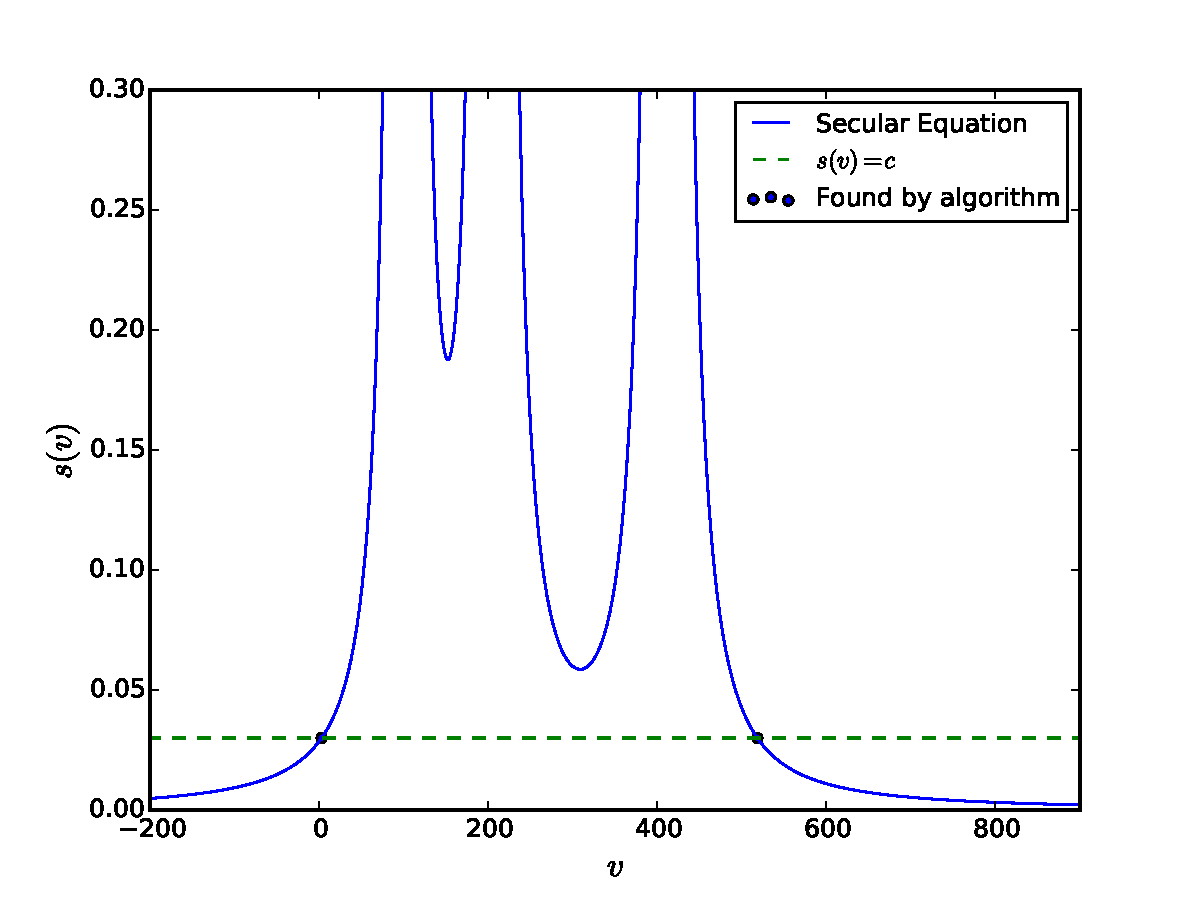
\includegraphics[trim=0in 0in 0.5in 0.5in,clip,width=1\linewidth]{images/secular}
\caption{Plot of secular equation for a single line in the RTS-96. Note that $s(v)$ approaches infinity at the three poles, and there could be as many as six solutions if $c$ were large enough.}
\label{fig:secular}
\end{figure}

%\begin{figure}
%\centering
%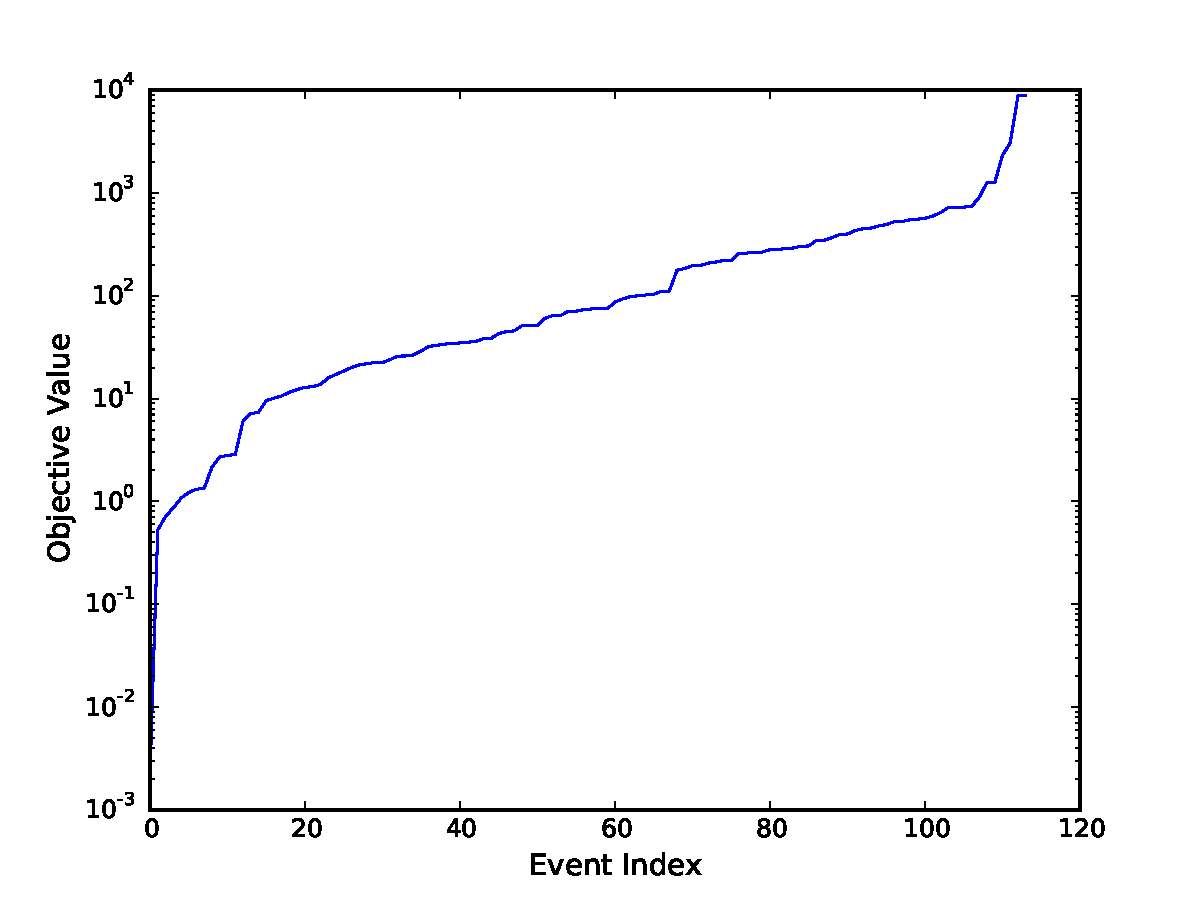
\includegraphics[width=1\linewidth]{../images/scores}
%\caption{Semilogarithmic plot of sorted objective values for RTS-96 temporal instanton analysis. (Note that six lines are missing objective values. The algorithm did not produce solutions for these lines due to numerical instability.)}
%\label{fig:scores}
%\end{figure}

%\begin{figure}[t]
%\centering
%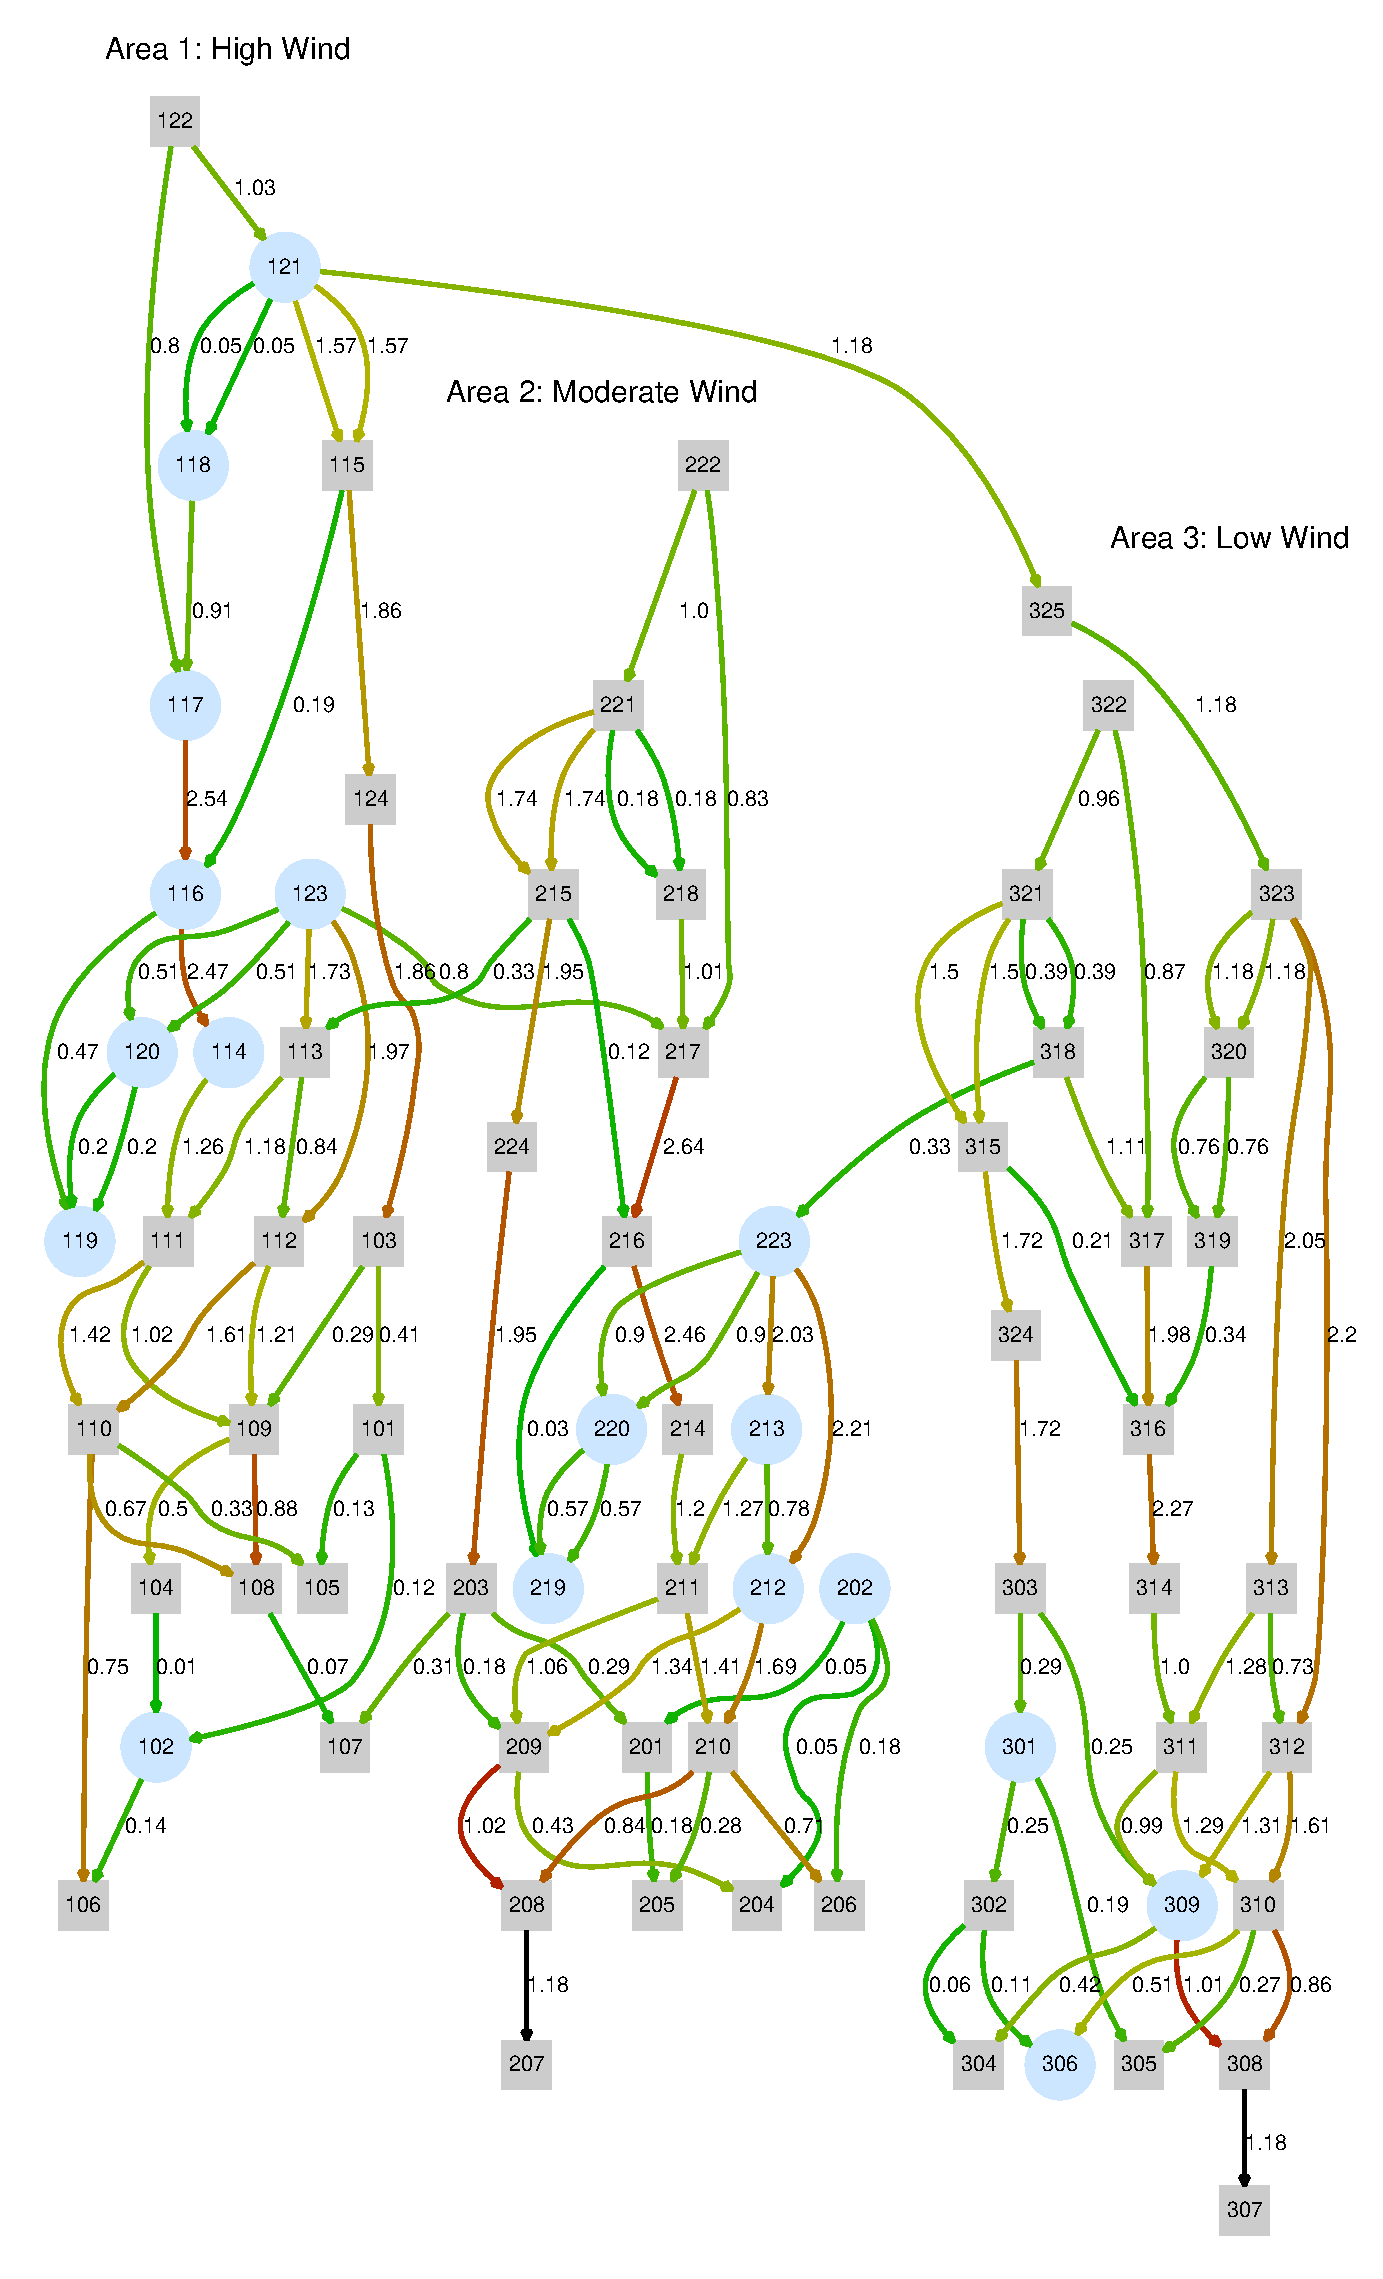
\includegraphics[width=1\linewidth]{images/line118}
%\caption{Graph depiction of RTS-96 system state under instanton conditions at time step 2 of 3. The stressed line is between buses 121 and 325 (top center). wind-farms are indicated by blue, and lines are colored according to how close their flows are to static active power limits.}
%\label{fig:line118}
%\end{figure}


\section{Conclusions}

%The paper has extended instanton analysis to consider the temperature
%dynamics of overloaded lines. The resulting formulation is a
%quadratically constrained quadratic program (QCQP)\@. A
%computationally cheap algorithm has been developed for obtaining
%candidate solutions of this QCQP\@.  There is a great deal of
%flexibility in the temporal instanton model that has yet to be
%explored. In future work we plan to include transformers, consider the
%effects of ambient conditions in greater detail, and test the limits
%of the algorithm using larger networks with many time steps.

\section{Appendix: line temperature model}\label{sec:temp}

\subsection{The heat balance equation}

The change in temperature of any object may be expressed as a differential equation called the heat balance equation, which relates temperature change to a sum of various sources of heating. The IEEE 738 standard \cite{ieee2013} provides the following heat balance equation for a transmission line:

\begin{align}\label{eq:heatbalance}
\frac{dT}{dt} &= \frac{1}{m\cdot C_p}\left[I^2\cdot R(T) - q_c - q_r + q_s \right]
\end{align}
where
\begin{itemize}
	\item $T$ is the conductor average temperature.
	\item $m\cdot C_p$ is the product of mass and heat capacity.
	\item $I^2\cdot R(T)$ represents heat rate due to resistive heating. In this paper the term is replaced by $f_{ij}^\text{loss}$, the DC approximate line loss expression derived in \cite{almassalkhi2014}:
	\begin{equation}
	\label{LL:activeLoss}
	f_{ij}^{\text{loss}} \approx r_{ij}\left(\frac{\theta_{ij}}{x_{ij}}\right)^2,
	\end{equation}
	where $\theta_{ij}$ is the difference between angles
	$\theta_i$ and $\theta_k$, and $r_{ij} +j x_{ij}$ is the impedance of
	the line between nodes $i$ and $j$. Three assumptions underpin
	\eqref{LL:activeLoss}: voltage magnitudes are all 1~pu, cosine may be
	approximated by its second-order Taylor expansion, and $x_{ij} \geq
	4r_{ij}$. Thus, \eqref{LL:activeLoss} uses DC power flow assumptions
	to approximate line losses, but remains nonlinear.
	\item $q_c$ is the rate of heat loss due to convection. Any object at a higher temperature than surrounding air will gradually cool as the air carries heat away. This phenomenon is proportional to the temperature difference between the line and surrounding air:
		\begin{align}\label{eq:qc}
		q_c &= \eta_c\cdot(T - T_\text{amb})~,
		\end{align}
	where $T_\text{amb}$ is the ambient temperature (of surrounding air).
	\item $q_r$ is the rate of heat loss due to radiation. Thermal radiation is the process by which thermal energy is converted to electromagnetic energy in all objects with non-zero absolute temperature. It is modeled by a fourth-order expression:
	  \begin{align}\label{eq:qr}
	    q_r &= \eta_r\cdot\left[(T + 273)^4 - (T_\text{amb} + 273)^4\right]
	  \end{align}
	\item $q_s$ is the rate of heat gain due to solar heating. In this paper the solar heat rate is fixed to some conservative constant (representing full direct sun), but it is important to note that solar heat rate varies significantly with cloud cover, geometry, and even insulation type (reflective versus black).
\end{itemize}
%\begin{align}\label{eq:738heatbalance}
%\frac{dT_\text{avg}}{dt} &= \frac{1}{mC_p}\left( r_{ij}\frac{\theta_{ij}^2}{x_{ij}^2}\frac{S_b}{3L_{ij}} - q_c - q_r + q_s\right)
%\end{align}

\subsection{Linearization of radiation heat rate}

When \eqref{eq:heatbalance} is combined with an initial temperature $T_0$, the resulting initial value problem makes it possible to determine the temperature at any later time. We substitute \eqref{eq:qc} and \eqref{eq:qr} into \eqref{eq:heatbalance} and attempt to solve for temperature:
\begin{multline}\label{eq:heatbalance_approx}
\frac{dT}{dt} = \frac{1}{mC_p}\big[ f_{ij}^\text{loss} - \eta_c\left( T(t) - T_\text{amb}\right) \\ - \eta_r\left((T(t) + 273)^4 - (T_\text{amb} + 273)^4\right) + q_s \big]
\end{multline}

Suppose that power flow, ambient temperature, and solar heat rate are constant during a temperature change calculation. Then there are just two variable terms on the right-hand side: one first-order and the other fourth-order. The fourth-order term (which comes from $q_r$) makes this equation difficult to solve. Fortunately, $q_r$ is approximately linear over the temperature range we are interested in (from ambient temperature to temperature limit). We replace $q_r$ by $\tilde{q}_r$, a conservative\footnote{Because a transmission line is hotter than surrounding air, radiation tends to decrease line temperature. Thus, a conservative approach will underestimate the radiation heat rate, leading to slightly higher temperatures.} linearization:
\begin{multline}\label{eq:approx_rad}
\tilde{q}_r = \eta_r  \left( (T_\text{mid} + 273)^4 - (T_\text{amb} + 273)^4\right) + \\ 4\eta_r(T_\text{mid} + 273)^3\cdot(T(t) - T_\text{mid})
\end{multline}
%\begin{figure}[h]
%\centering
%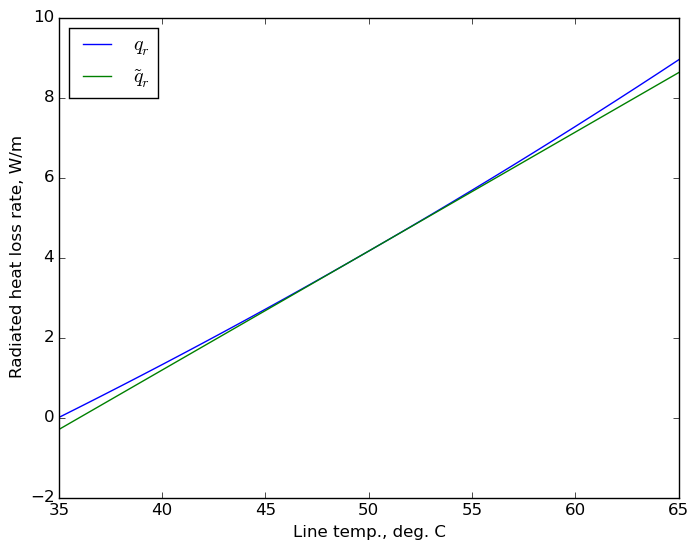
\includegraphics[width=0.9\linewidth]{../images/rad_approx}
%\caption{Comparison of fourth-order radiation heat rate $q_r$ \eqref{eq:qr} with conservative linearization $\tilde{q}_r$ across a range of temperatures. Ambient temperature is 35$^\circ$C and the conductor thermal limit is 65$^\circ$C.}
%\label{fig:rad_approx}
%\end{figure}
%
%The green trace is the linearization of $q_r$ about $T_\text{mid}$, the midpoint between the ambient and limit temperatures. Let's replace $q_r$ by this linear approximation $\tilde{q}_r$:

\subsection{Line temperature as recursive relationship}
Substitution of \eqref{eq:approx_rad} into \eqref{eq:heatbalance_approx} yields the approximate heat balance equation
\begin{align}\label{eq:diffeq}
\frac{dT}{dt} &= aT(t) + b~,
\end{align}
where constants $a$ and $b$ are defined as
\begin{subequations}
\begin{align}
a &= \frac{1}{mC_p} \left[ -\eta_c - 4\eta_r(T_\text{mid} + 273)^3 \right]
\end{align}
\begin{multline}
b = \frac{1}{mC_p} \big[ f_{ij}^\text{loss} + \eta_cT_\text{amb} - \eta_r \big( (T_\text{mid} + 273)^4 \\ - (T_\text{amb} + 273)^4 \big) + 4\eta_rT_\text{mid}(T_\text{mid} + 273)^3 + q_s \big]
\end{multline}
\end{subequations}

Our approximate heat balance initial value problem \eqref{eq:diffeq} has a straightforward solution:

\begin{align}\label{eq:tivp}
T(t) &= ke^{at} - \frac{b}{a}
\end{align}

where $k=T(0) + b/a$. Note that $b$ is influenced by power flow (via
$f_{ij}^\text{loss}$), but $a$ is not.

The only variables in \eqref{eq:tivp} are initial temperature and angle differences during each time interval. There is therefore a recursive relationship between final temperature and initial temperature that involves only angle differences. The derivation of this recursive relationship is an exercise in messy linear algebra; it is omitted here for brevity.
%Suppose there are three time intervals: $t_1$, $t_2$, and $t_3$. Then the line temperature at the end of the third interval is given by
%
%\begin{align}
%\nonumber T(t_3) &= k_3 e^{(t_3-t_2)a} - \frac{b_3}{a} \\
%\nonumber &= \left[k_2 e^{(t_2-t_1)a} - \frac{b_2}{a} + \frac{b_3}{a}\right]e^{(t_3-t_2)a} - \frac{b_3}{a} \\
%\nonumber &= \left[\left( T(t_1) + \frac{b_2}{a} \right)e^{(t_2-t_1)a} - \frac{b_2}{a} + \frac{b_3}{a}\right]e^{(t_3-t_2)a} - \frac{b_3}{a} \\
%\label{eq:Texpand} &= \Bigg\lbrace\left[\left(T(t_0) + \frac{b_1}{a}\right) \nonumber e^{(t_1-t_0)a} - \frac{b_1}{a} + \frac{b_2}{a}\right]e^{(t_2-t_1)a} \\
%& \qquad \qquad \qquad \qquad - \frac{b_2}{a} + \frac{b_3}{a}\Bigg\rbrace e^{(t_3-t_2)a} - \frac{b_3}{a}
%\end{align}
%The recursive pattern is apparent. Because all time intervals are the same length, we have
%\begin{align*}
%e^{(t_3-t_2)a} &= e^{(t_2-t_1)a} = e^{(t_1-t_0)a}~,
%\end{align*}
%and we can distribute in \eqref{eq:Texpand} to obtain
%\begin{multline}
%T(t_3) = (e^{(t_1-t_0)a})^3\left(T(t_0) + \frac{b_1}{a}\right) \\ + (e^{(t_1-t_0)a})^2\left(- \frac{b_1}{a} + \frac{b_2}{a}\right) \\ + (e^{(t_1-t_0)a})\left(- \frac{b_2}{a} + \frac{b_3}{a}\right) - \frac{b_3}{a}
%\end{multline}
%Because power flow data enters through $b_1$, $b_2$, and $b_3$, it makes sense to
%group terms accordingly:
%
%\begin{multline}
%T(t_3) = ((e^{(t_1-t_0)a})^3T(t_0) + \\ \left(\frac{(e^{(t_1-t_0)a})^3}{a} - \frac{(e^{(t_1-t_0)a})^2}{a}\right)b_1 \\ + \left( \frac{(e^{(t_1-t_0)a})^2}{a} - \frac{(e^{(t_1-t_0)a})^1}{a}\right)b_2 \\ + \left(\frac{e^{(t_1-t_0)a}}{a} - \frac{1}{a}\right) b_3
%\end{multline}
%The pattern in the above expression makes it easy to extend $T(t_3)$ to cover the general case $T(t_n)$:
%
%\begin{multline}\label{eq:recursive}
%T(t_n) = (e^{(t_1 - t_0)a})^n T(t_0) \\ + \frac{1}{a} \sum_{i=1}^n \left( (e^{(t_1-t_0)a})^i - (e^{(t_1-t_0)a})^{i-1} \right)b_{n-i+1}
%\end{multline}
%
%Ultimately \eqref{eq:recursive} will be used to constrain a line's final temperature to some limiting value. The remainder of this section will relate \eqref{eq:recursive} back to power flow angles so it can be ``plugged in'' to the optimization framework.
%
%\subsection{Relating temperature to angle differences}
%
%Recall that $b_n$ depends on the angle difference at time $t_n$:
%
%\begin{align}
%\nonumber b_n &= \frac{1}{mC_p} \Bigg[ \frac{r_{ij}}{x_{ij}^2}\cdot \frac{S_b}{3L_{ij}} \theta_{ij}(t_n)^2 + \eta_cT_\text{amb} \\
%\nonumber &\qquad - \eta_r\left((T_\text{mid} + 273)^4 - (T_\text{amb} + 273)^4\right) \\
%&\qquad + 4\eta_rT_\text{mid}(T_\text{mid} + 273)^3 + q_s \Bigg] \\
%\label{eq:bexpand} b_n &= c\theta_{ij}(t_n)^2 + d
%\end{align}
%where constants $c$ and $d$ are defined as:
%\begin{align*}
%c &= \frac{r_{ij}S_b}{3 mC_p x_{ij}^2L_{ij}} \\
% d &= \frac{1}{mC_p}\left[ \eta_cT_\text{amb} - \eta_r\left((T_\text{mid} + 273)^4 - (T_\text{amb} + 273)^4\right) + 4\eta_rT_\text{mid}(T_\text{mid} + 273)^3 + q_s \right]
%\end{align*}
%Substitute \eqref{eq:bexpand} into \eqref{eq:recursive}:
%\begin{align*}
%T(t_n) &= (e^{(t_1 - t_0)a})^n T(t_0) + \frac{1}{a} \sum_{i=1}^n \left( (e^{(t_1-t_0)a})^i - (e^{(t_1-t_0)a})^{i-1} \right)(c\theta_{ij}(t_{n-i+1})^2 + d)
%\end{align*}
%Expand the sum term:
%\begin{multline}\label{eq:sumexpand}
%\frac{1}{a} \sum_{i=1}^n \left( (e^{(t_1-t_0)a})^i - (e^{(t_1-t_0)a})^{i-1} \right)(c\theta_{ij}(t_{n-i+1})^2 + d) = \frac{c}{a}\left[ \sum_{i=1}^n \left( (e^{(t_1-t_0)a})^i - (e^{(t_1-t_0)a})^{i-1} \right)\theta_{ij}(t_{n-i+1})^2\right] + \\  \qquad + \frac{d}{a}\left[ \sum_{i=1}^n \left( (e^{(t_1-t_0)a})^i - (e^{(t_1-t_0)a})^{i-1} \right)\right]
%\end{multline}
%Substitute \eqref{eq:sumexpand} into the line temperature equation, introducing the constant $f$ to keep things a bit neater:
%\begin{align}\label{eq:almostthere}
%T(t_n) &= f + \frac{c}{a}\left[ \sum_{i=1}^n \left( (e^{(t_1-t_0)a})^i - (e^{(t_1-t_0)a})^{i-1} \right)\theta_{ij}(t_{n-i+1})^2\right]
%\end{align}
%where
%\begin{align}
%f &= (e^{(t_1 - t_0)a})^n T(t_0) + \frac{d}{a}\left[ \sum_{i=1}^n \left( (e^{(t_1-t_0)a})^i - (e^{(t_1-t_0)a})^{i-1} \right)\right]
%\end{align}
%Rearrange \eqref{eq:almostthere} to isolate angle differences:
%\begin{align}
%\sum_{i=1}^n \left( (e^{(t_1-t_0)a})^i - (e^{(t_1-t_0)a})^{i-1} \right)\theta_{ij}(t_{n-i+1})^2 &= \frac{a}{c}(T(t_n) - f)
%\end{align}
%Now define
%\begin{equation}\label{eq:thetahat}
%\hat{\theta}_{ij}(t_{k})=  \theta_{ij}(t_k)\sqrt{ (e^{(t_1-t_0)a})^{n-k+1} - (e^{(t_1-t_0)a})^{n-k} }
%\end{equation}
%to obtain
%\begin{align}\label{eq:finaltemp}
%\sum_{k=1}^n \hat{\theta}_{ij}(t_{k})^2 &= \frac{a}{c}\left(T(t_n) - f\right)
%\end{align}
%The expression \eqref{eq:finaltemp} may be used to constrain line temperature to be equal to some limiting value by the end of the last time interval.
%
%This derivation has been somewhat messy. The line temperature constraint is summarized in the next section for convenience.




%Comparison with the temperature calculation method recommended by IEEE in \cite{ieee2013} shows th To validate the approximate line temperature model derived here, I compared it to the IEEE 738 standard model using RTS-96 and Waxwing conductor parameters.
%
%\subsection{Summary of IEEE 738 temperature calculation}\label{summary-of-ieee-738-temperature-calculation}
%
%IEEE recommends numerically integrating \eqref{eq:heatbalance} to compute temperature changes. The temporal instanton framework uses approximate DC losses in place of $I^2R(T_\text{avg})$, so we will be integrating the following heat balance equation:
%
%\begin{align}\label{eq:738heatbalance}
%\frac{dT_\text{avg}}{dt} &= \frac{1}{mC_p}\left( r_{ij}\frac{\theta_{ij}^2}{x_{ij}^2}\frac{S_b}{3L_{ij}} - q_c - q_r + q_s\right)
%\end{align}
%
%Heat rates $q_c$ and $q_r$ are calculated according to \eqref{eq:qc} and \eqref{eq:qr}, respectively (copied here for convenience):
%\begin{align*}
%q_c &= \eta_c\cdot(T - T_\text{amb}) \\
%q_r &= \eta_r\cdot((T + 273)^4 - (T_\text{amb} + 273)^4)
%\end{align*}
%All other parameters are constant during temperature calculation. The important thing to keep in mind about IEEE 738 temperature calculation is that it requires numerical integration; there is no analytic temperature solution for \eqref{eq:738heatbalance}. This means one must select an integration time step $\Delta t$. For each step, one computes the change in temperature by multiplying $\Delta t$ by the value of \eqref{eq:738heatbalance} computed at that step. IEEE recommends a step size smaller than 10\% of the conductor thermal time constant\footnote{A typical transmission line thermal time constant is ten minutes, which means IEEE recommends an integration step size of one minute}. A smaller integration step size yields more accurate results.
%
%\subsection{Comparison}\label{comparison}
%
%I used RTS-96 network data and Waxwing conductor parameters to compare IEEE 738 standard temperature calculation to the model derived in Section \ref{transmission-line-heating}. Figure \ref{fig:temp_model_comparison2} shows line temperatures calculated across three ten-minute time intervals, where each interval has a different angle difference (power flow). The angle differences are
%\begin{center}
%\begin{tabular}{c|c}
%	Interval & Angle difference (rad) \\ \hline
%	   1     &          0.09          \\
%	   2     &          0.04          \\
%	   3     &          0.15          \\
%\end{tabular}
%\end{center}
%
%\begin{figure}[h]
%\centering
%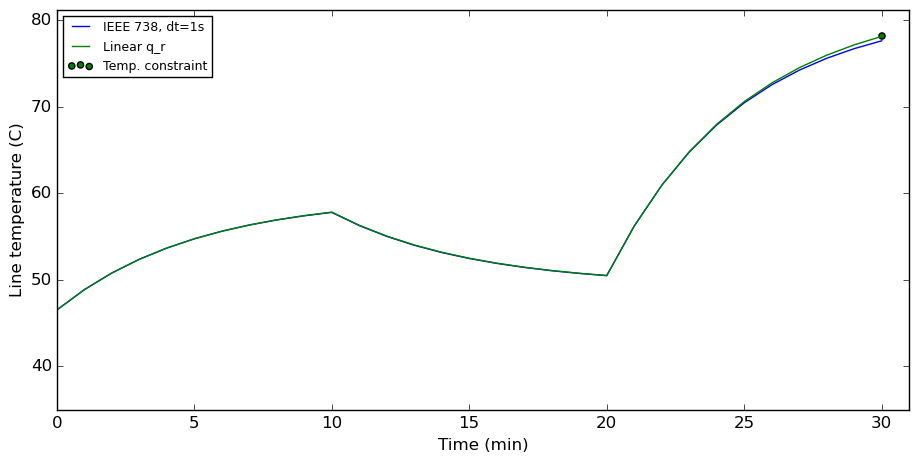
\includegraphics[width=1\linewidth]{../images/temp_model_comparison2}
%\caption{Comparison of IEEE 738 and approximate temperature calculation methods}
%\label{fig:temp_model_comparison2}
%\end{figure}
%
%The blue trace in Figure \ref{fig:temp_model_comparison2} results from numerical integration of \eqref{eq:738heatbalance} with a 1s step size. The green trace comes from the approximate model derived in Section \ref{transmission-line-heating}. The green dot is the final temperature computed by \eqref{eq:almostthere}.
%
%Notes:
%
%\begin{itemize}
%\item
%  Because the approximate line temperature model is analytic (Equation \eqref{eq:tivp} is continuous) while the 738 model requires numerical integration, I chose
%  a very small integration step size of one second to facilitate comparison.
%\item
%  Because the approximate model underestimates the radiative heat loss
%  rate (see Figure \ref{fig:rad_approx}), the green trace should lie slightly above the blue one. This
%  makes the approximate model conservative, which is desirable in the
%  temporal instanton setting. Figure \ref{fig:temp_model_comparison2} illustrates this conservative behavior: the green trace lies on or above the blue trace throughout the time horizon.
%  \item The green dot, computed by \eqref{eq:almostthere}, lies on top of the green curve. This validates the temperature constraint formulation \eqref{eq:tempconstraint}.
%\end{itemize}


%Section \ref{sec:line-losses} describes an approximate line loss formulation that forms the basis of a dynamical model developed in Section \ref{sec:temp-dynamics}. Finally, Section \ref{sec:instanton-formulation} incorporates line temperature dynamics into a complete mathematical model.

%The equations governing AC power flow are nonlinear. If we use these equations to balance the power flows in our optimization, the resulting feasible region will be nonconvex. Previous instanton work has addressed this issue by replacing the AC power flow equations with DC equations (the DC power flow equations assume that the network is lossless, with all voltage magnitudes equal to 1 per unit). This substitution renders the feasible region of instanton optimization (in the absence of nonlinear constraints) convex.

%There are two primary difficulties associated with time-coupled instanton analysis. First, every active and reactive power flow is related to all variables involved in the flow:  the voltage magnitudes at both nodes and the angle difference between them. If we allow this tight coupling into our optimization framework, there will be no guarantee of a unique solution, or indeed of any solution at all. The second difficulty arises from the equation for power loss. Power loss on a line is proportional to the square of the current through it. This nonlinear relationship leads to nonconvexity in the optimization problem's feasible region. In this paper we address the first concern by using the DC power flow, and we sidestep the second difficulty by using a piecewise-continuous convex relaxation of the power loss equation.


\newcommand{\splitcell}[2][c]{%
\begin{tabular}[#1]{@{}c@{}}#2\end{tabular}}
\begin{table}
\begin{center}
\caption{Line heating parameters}
\label{tab:heatparams}
\begin{tabular}{|c|c|c|}
	\hline
	         Parameter           &   Units    &               Description                \\ \hline
	           $T_s$             &    $s$     &               Sample time                \\ \hline
	           $mC_p$            & $J/(m\cdot C)$ & \splitcell{Per-unit-length heat capacity\\of the conductor}         \\ \hline
	          $\eta_c$           & $W/(m\cdot C)$ &     \splitcell{Conductive heat loss \\ rate coefficient}         \\ \hline
	          $\eta_r$           & $W/(m\cdot C)$ &      \splitcell{Radiative heat loss\\rate coefficient}         \\ \hline
	       $T^\text{lim}$        &    $C$     &      \splitcell{Line temperature at\\steady-state current limit.}   \\ \hline
	       $\Delta q_{s,ij}$ & $W/m$ & \splitcell{Solar heat input\\ into conductor} \\ \hline
	       $\Delta T_\text{amb}$ & C & \splitcell{Change in \\ambient temperature} \\ \hline
\end{tabular}
\end{center}
\end{table}



% The paper will close with a discussion of how other
%components, such as voltage regulators, may affect the formulation.

%\section*{Acknowledgment}

%\section*{References}

% can use a bibliography generated by  as a .bbl file
% BibTeX documentation can be easily obtained at:
% http://www.ctan.org/tex-archive/biblio/bibtex/contrib/doc/
% The IEEEtran BibTeX style support page is at:
% http://www.michaelshell.org/tex/ieeetran/bibtex/
\bibliographystyle{IEEEtran}
% argument is your BibTeX string definitions and bibliography database(s)
%\bibliography{IEEEabrv,../bib/paper}
\bibliography{bib}

\end{document}
